\subsection{Representation Learning}\label{sec:dl}
Representation Learning or in common words Deep learning can be considered as a subset of machine learning but has gained attention as a different field due to its success in various vision, text and speech tasks. The difference about deep learning that makes it perform better on various complex problems is that it doesn't require domain expertise to identify the features to represent a problem or case from previous experience. Instead it automatically learns the features during training process using a large set of training data on various iterations. 

Initially deep learning outperformed a lot of state-of-the-art algorithms in vision tasks and established itself as the benchmark solutions \cite{simonyan2014very,he2016deep}, but during the past few years with the advancement in computing powers and the availability of large datasets the \textbf{``The Deep Learning Tsunami''} \cite{manning2015computational} has taken over NLP as well. In this section we will sequentially talk about the development of deep learning applied in NLP to solve the various tasks.

\subsubsection{Word Embeddings} \label{sec:word_emb}
When using deep learning and to solve an NLP task, each word in the vocabulary is represented in a vector form so that it can be fed into the neural networks. Word embedding is the way of converting a word $w_{i}$ in vocabulary $V$ in the form of a vector of $n$ dimensions. These word vectors are generated by unsupervised training on a large corpus of words in order to gain the semantic similarities between the words. Algorithms like word2vec \cite{mikolov2013distributed} and GloVe \cite{pennington2014glove} are used to train these word embeddings. These word embeddings are generally pre-trained and made available to be downloaded from the internet and used directly in the deep learning models.

These distributed representation of words give a certain amount of semantic understanding of the words in a high dimensional vector space. For example, the distance between words $king$ and $queen$ will be similar to the distance between $boy$ and $girl$. In this contrast the \cref{eq:we1} fits perfectly. 
% A visualization of these word embeddings in low dimension is shown in \cref{fig:glove_ex} \footnote{taken from \url{http://web.stanford.edu/class/cs224n/}}.

\begin{equation}\label{eq:we1}
    boy - girl + king = queen
\end{equation}

% \begin{figure}
%     \centering
%     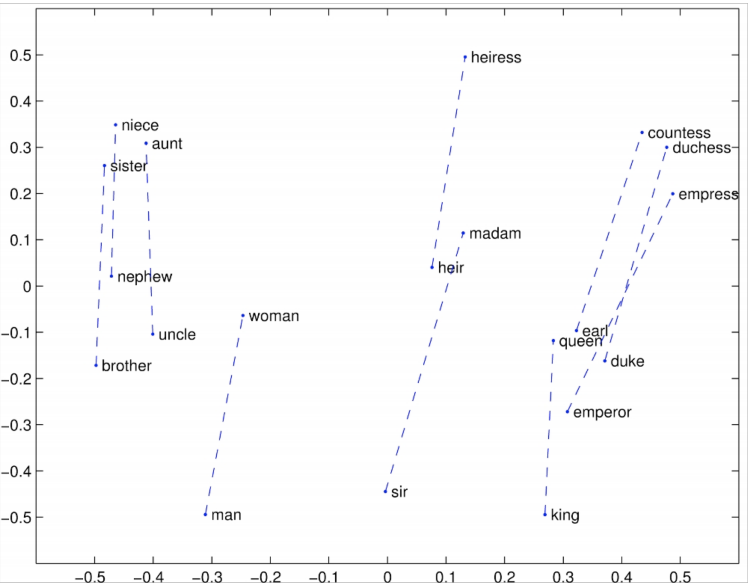
\includegraphics[width=0.5\textwidth]{images/glove_vecs.png}
%     \caption{GloVe words visualization in 2D space}
%     \label{fig:glove_ex}
% \end{figure}

These representations have a drawback that they fail to take context of a word into account. For example, the word \textit{`Scotland'} will have a different meaning in the sentence \textit{`Scotland is one of the most best places to live on earth'} than in the sentence \textit{`Royal Bank of Scotland is one of the top banking firms in the UK'}. The glove or word2vec word embedding will fail to differentiate the two meanings of Scotland and will assign same vector in both the cases. These drawbacks are tackled by a new concept of contextual word embeddings discussed in \cref{sec:context_we}

\subsubsection{Language Models}\label{sec:lm}

\begin{figure}
    \centering
    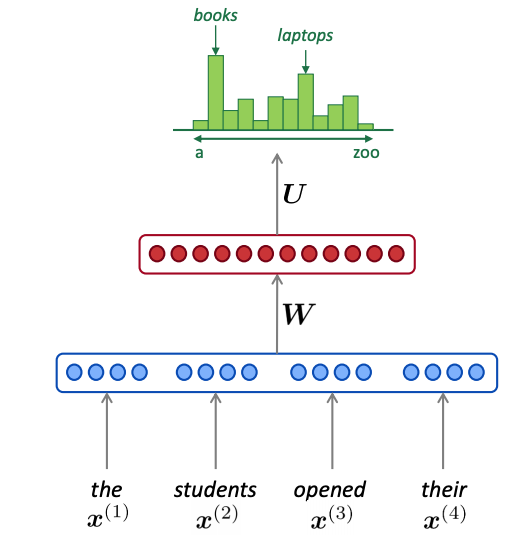
\includegraphics[width=0.45\textwidth]{images/lang_model.png}
    \caption{Prediction of next word using a Language Model}
    \label{fig:lang_model}
\end{figure}

A language model is a type of system that predicts the probability of possible next words given a sequence of words as the input. In general terms, for a given sequence of input $(x_{1}, x_{2}, \cdots, x_{t})$, the probability distribution of next term $x_{t+1}$ is computed from a vocabulary $V$ of $k$ words ($V = (w_{1}, w_{2}, \cdots, w_{k})$). 

\begin{equation}
    \label{eq:lm_dist}
        P(x_{t+1}|x_{1}, \cdots, x_{t})
\end{equation}

Earlier the language models were based on statistical approaches where they used to take a window of $n$ words as a context from the sentence to predict the next word. This approach is also known as $ngram$ Language Model. It takes an simple approach of calculating the conditional probability of next word in the sentence given the window of $n$ words as a context. These $ngram$ probabilities are calculated from counting them in some large corpus of text.

\begin{equation}
    \label{eq:lm_ngram}
        P(x_{t+1}|x_{1}, \cdots, x_{t}) = 
            \frac {P(x_{t+1}, x_{t}, \cdots, x_{t-n+2})} {P(x_{t}, \cdots, x_{t-n+2})}
\end{equation}

or in simpler terms:

\begin{equation}
    \label{eq:lm_count_ngram}
        P(w_{3}|w_{1},w_{2}) = \frac{count(w_{1}, w_{2}, w_{3})}{count(w_{1}, w_{2})}
\end{equation}

This statistical approach has mainly two problems. First sparsity, consider the \cref{eq:lm_count_ngram}, what if $w_{1}$, $w_{2}$ and $w_{3}$ never occurred together. The probability of $w_{3}$ will be 0. Also, if $w_{1}$ and $w_{2}$ then there's no way to calculate the probability of $w_{3}$. Second storage, as we increase the value of $n$, the count of all $nrgams$ we see in the corpus increases as well and so does the need of memory to store them.

The neural language model using Recurrent Neural Networks (\cref{sec:rnn}) were able to model all the words in a sentence without having a need of window to predict the next word at each timestep using hidden state and output from the previous time step combining with the new input at each time step. 


\subsubsection{Recurrent Neural Networks} \label{sec:rnn}
Text is a sequential form of data. To process text and extract information we need a model capable of processing the sequential data. \textit{Recurrent Neural Networks} \cite{elman1990finding} are the most elementary deep learning architectures that are able to learn from sequential data. RNN, are wide in nature as they unroll through time. These networks will have a `memory' component which can store the information about previous state. They share same set of weights throughout the layers, however, will receive a new input at every layer or time-step. The output to every time-step is dependent on the input taken at the current time-step $t_{i}$ as well as the information gained from previous time-step $t_{i-1}$. Specifically, an RN Net will maintain a hidden state $h_{t}$ at every step which is referred as the memory of network. An illustrated diagram of unrolled RNN is shown in fig \cref{fig:rnn_unrolled} \footnote{taken from \url{https://colah.github.io/posts/2015-08-Understanding-LSTMs/}}.

\begin{figure}
    \centering
    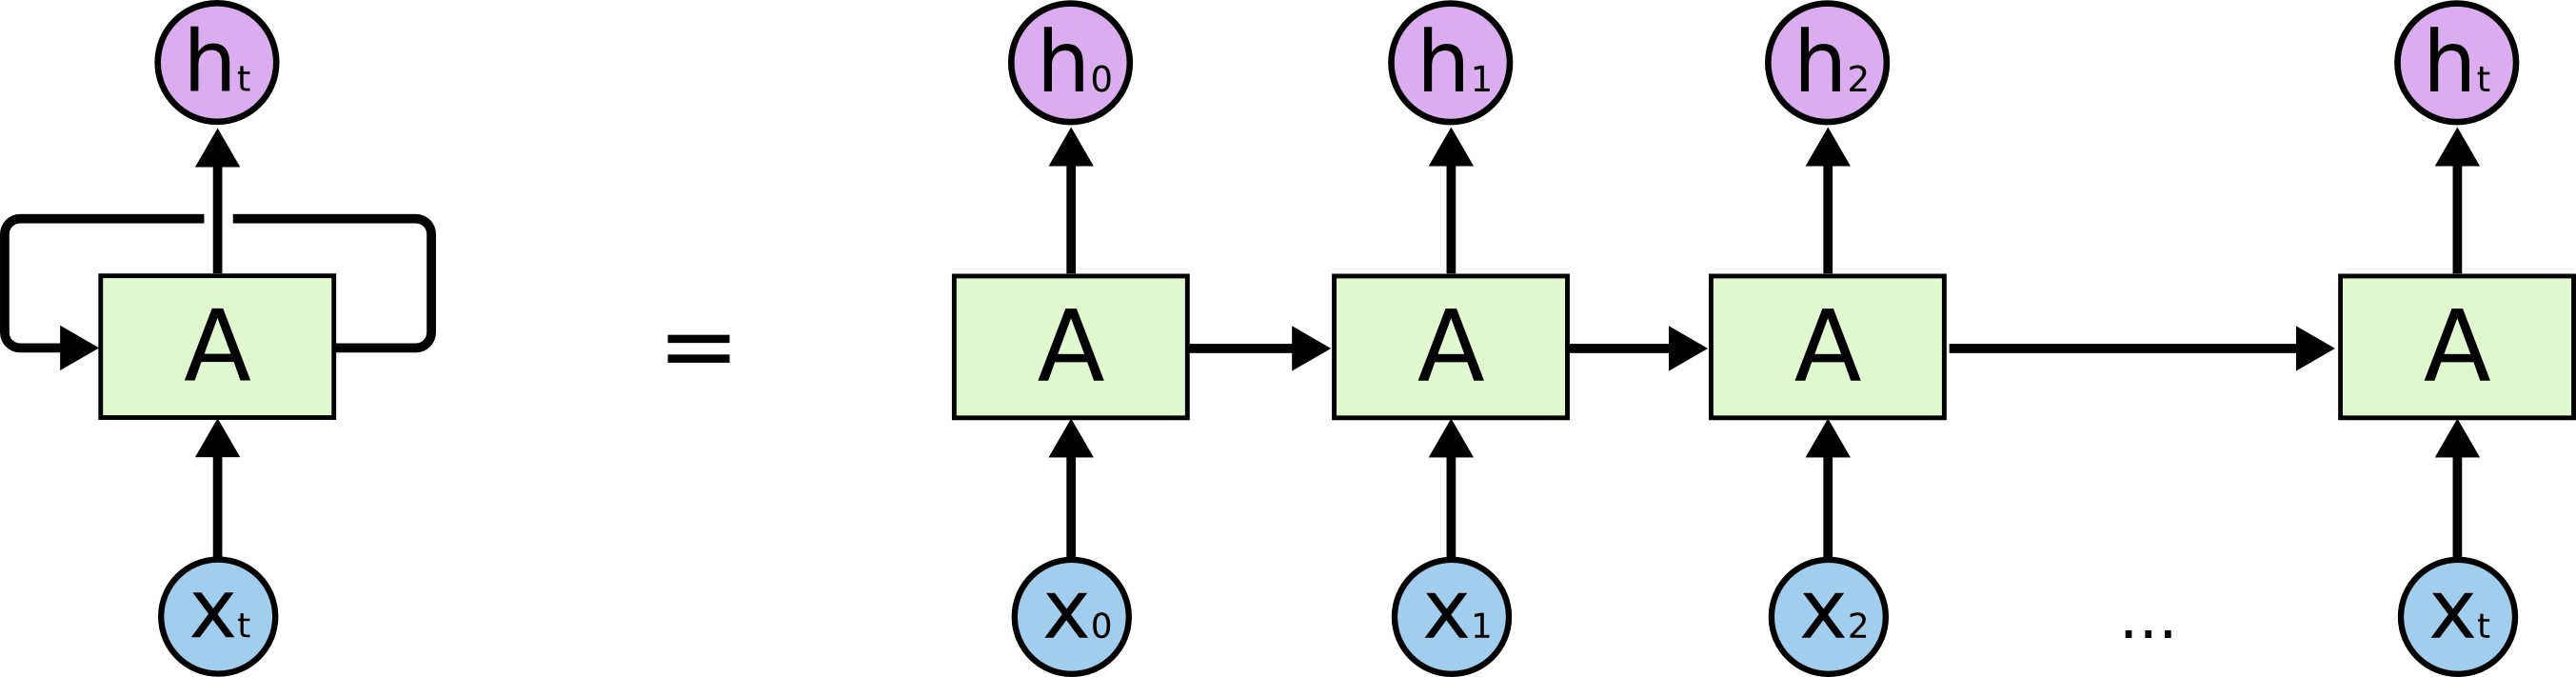
\includegraphics[width=\textwidth]{images/RNN-unrolled.png}
    \caption{RNN Unrolled}
    \label{fig:rnn_unrolled}
\end{figure}

The operations performed in RNN at every time step is given in the \cref{eq:rnn}.

\begin{align}\label{eq:rnn}
    \begin{gathered}
        h_{t} = \sigma_{h}(W_{e}x_{t} + W_{h}h_{t-1} + b_{h}) \\
        y_{t} = \sigma_{y}(W_{y}h_{t} + b_{y})
    \end{gathered}
\end{align}

Here $\sigma_{y}$ and $\sigma_{h}$ are the activation functions. $W_{h}$ is the weight matrix to apply transformation on previous hidden state $h_{t-1}$, $W_{e}$ is the weight matrix to apply transformation on the input $x_{t}$ received over time $t$. Combining these with the bias $b_{h}$ yields hidden state $h_t$ for time $t$. Applying activation on the $h_{t}$ with $W_{y}$ gives the output $y_t$ for every time-step $t$.


\subsubsection{Long Short-Term Memory Networks}
Although, in theory the RNNs are designed to handle the sequence input but in practice they lack in storing the long term dependencies because of the problem of exploding and vanishing gradients \cite{bengio1994learning}. Long Short-Term Memory Networks \cite{hochreiter1997long} are the advanced version of RNNs with a slight modification of being capable of deciding what to `remember' and what to `forget' from the input sequence with the help of a series of gates. LSTM has a number of gates, an output gate, an input gate $i_{t}$, forget gate $f_{t}$, $o_{t}$, all of which are the functions of previous hidden state $h_{t}$ and current input $x_{t}$. These gates interact with the previous cell state $c_{t-1}$, the current input $x_{t}$, and the current cell state $c_{t}$ and enable the model to selectively retain or information from the sequence. The full version of LSTM is given in the \cref{eq:lstm}.

\begin{equation}\label{eq:lstm}
    \begin{gathered}    
        f_{t} = \sigma_{g} (W_{f}x_{t} + U_{f}h_{t-1} + b_{f}) \\
        i_{t} = \sigma_{g} (W_{i}x_{t} + U_{i}h_{t-1} + b_{i}) \\
        o_{t} = \sigma_{g} (W_{o}x_{t} + U_{o}h_{t-1} + b_{o}) \\
        \Tilde{c_{t}} = \sigma_{c} (W_{c}x_{t} + U_{c}h_{t-1} + b_c)\\
        c_{t} = f_{t} \circ c_{t-1} + i_{t} \circ \Tilde{c_{t}}\\
        h_{t} = o_{t} \circ \sigma_{h}(c_{t})
    \end{gathered}
\end{equation}

where $\sigma_{g}$ is the $sigmoid$ activation function, $\sigma_{c}$ and $\sigma_{h}$ are the $tanh$ activation function, and $\circ$ is element-wise multiplication, also known as \textit{`Hadamard product'}. An illustrated diagram of unrolled RNN is shown in fig \cref{fig:lstm} \footnote{taken from \url{https://colah.github.io/posts/2015-08-Understanding-LSTMs/}}.

\begin{figure}
    \centering
    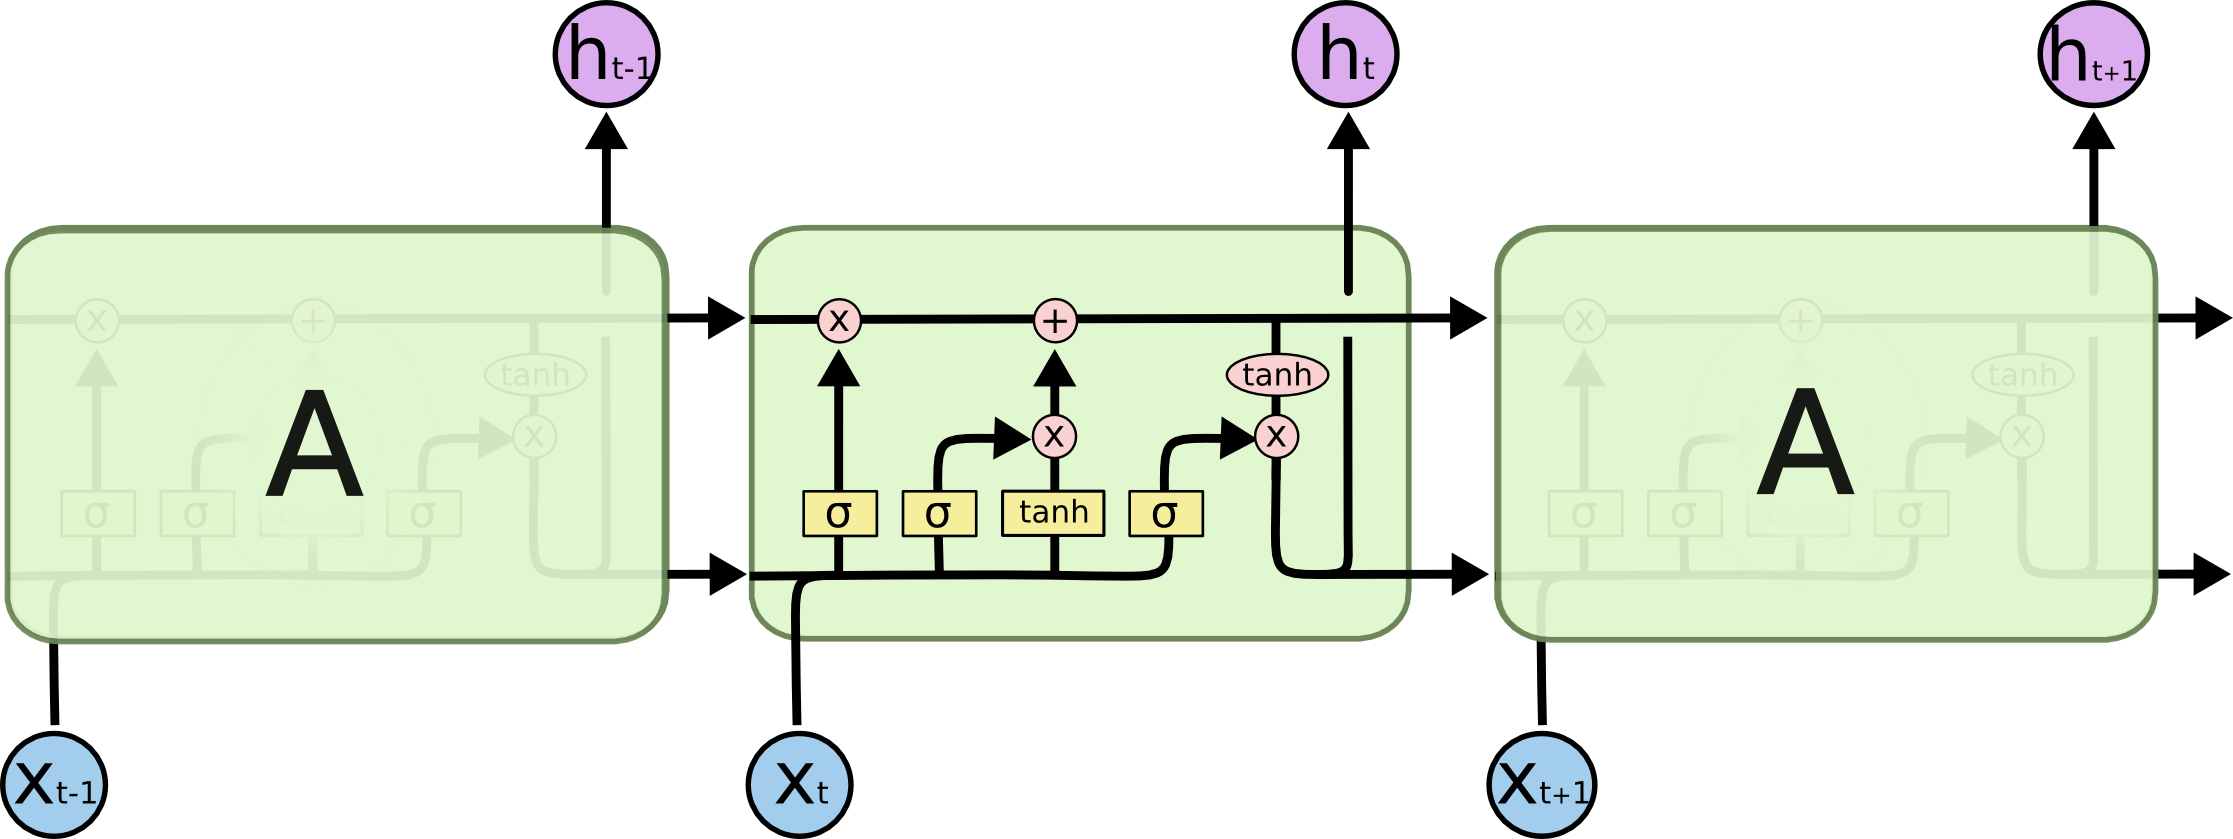
\includegraphics[width=\textwidth]{images/lstm.png}
    \caption{LSTM}
    \label{fig:lstm}
\end{figure}

LSTM layers can be stacked on each other to form multiple layer LSTM architecture. One of the most popular LSTM architecture is Bidirectional LSTM (BiLSTM) \cite{graves2013hybrid}, where two separate LSTMs are ran forward and backward to gain the sequential information in both directions.

\subsubsection{Convolutional Neural Networks}
Convolutional Neural Networks \cite{lecun1998gradient} are the version of deep neural networks established as state-of-the-art in various computer vision tasks \cite{barbu2019objectnet,ali2019mfc}. After the release of AlexNet \cite{krizhevsky2012imagenet} in ImageNet competition 2012, CNNs have been the benchmark for almost every vision task. Inspired from the popularity of CNN in vision, researchers proposed an CNN architecture for sentence classification which outperformed many benchmarks on various text classification dataset ranging from sentiment analysis to topic classification \cite{kim2014convolutional}. 

\begin{figure}
    \centering
    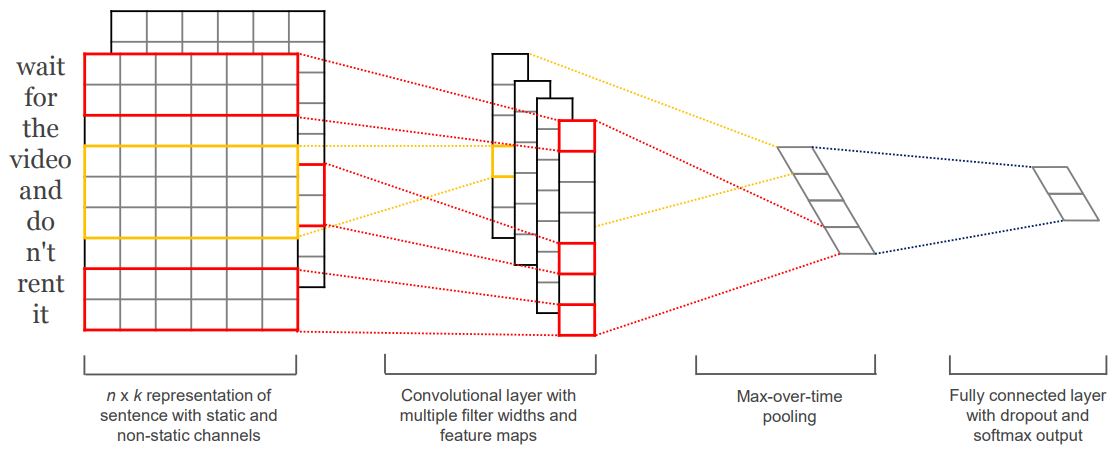
\includegraphics[width=\textwidth]{images/cnn_text.png}
    \caption{CNN for sentence classification}
    \label{fig:cnn}
\end{figure}

CNNs are capable of computing vectors for all possible sub-phrases in a sentence, not just grammatically correct one as done by RNNs. A CNN takes an input sentence of word length $n$ where each word is represented distributively in $d$ dimension. So the input $X_{1:n}$ is a $2D$ matrix of shape $n \times d$  where $x_{i}$ $\epsilon$ $\mathbb{R}^d$. Input $X_{1:n}$ can be represented as \cref{eq:cnn_input}.

\begin{equation}
    \label{eq:cnn_input}
    X_{1:n} = x_{1} \oplus x_{2} \oplus \cdots \oplus x_{n}
\end{equation}

where $\oplus$ is the concatenation operator. On the input layer, convolution filter $W$  $\epsilon$ $\mathbb{R}^{hd}$ is applied over window of $h$ words to generate a new feature. So, a feature $c_{i}$ is generated from the word window $x_{i:i+h-1}$ with the following operation:

\begin{equation}
    c_{i} = \sigma (Wx_{i:i+h-1} + b)
\end{equation}

where $W$ is the weight matrix for the connections, $\sigma$ is the activation function and $b$ $\epsilon$ $\mathbb{R}$ is the bias. Now, this filter is applied to each possible window of words giving an feature map $C$ $\epsilon$ $\mathbb{R}^{n-h+1}$.

\begin{equation}
    C = [c_{1}, c_{2}, \cdots, c_{n-h+1}]
\end{equation}

The entries in feature map $C$ are sharing the parameter $W$, where each $c_{i}$ $\epsilon$ $C$ is a result of calculation on small segment of the input. Then a $max-pooling$ operation is applied on these feature maps to capture the most important part.

\begin{equation}
    \Tilde{C} = max(C)
\end{equation}

This parameter sharing helps the model to incorporate an inductive bias into the model, helping to become learn the location invariant local features. There are $k$ number of filters applied to the input with different window sizes which are then concatenated to form a vector $\textbf{K}$ $\epsilon$ $\mathbb{R}^k$. Which is then fed to next hidden layer or output layer.

An illustrated diagram of an CNN architecture for text classification is shown in fig \cref{fig:cnn} \footnote{taken from \cite{kim2014convolutional}}.

\subsubsection{Sequence  to Sequence Models}
Most of the NLP tasks require sequential output instead of a single output label unlike classification or regression \cite{sutskever2014sequence}. These tasks can be Machine Translation of natural language, Question-Answering or Summary generation systems. These systems take a sequence of input and process it to produce yet another sequence for output. The goal is to take a sequence $(x_{1}, x_{2}, \cdots, x_{n})$ as input and map it to another sequence $(y_{1}, y_{2}, \cdots, y_{n})$ as output.

The architecture used to deal with these kind of problems is known as Sequence to Sequence model or in common terms, seq2seq model. It is a combination of auto-encoders and decoders which works in a sequential manner where encoder is an neural architecture to generate a context vector from input sequence and decoder, another neural architecture taking context vector as input and generating the output sequence.

The encoder takes an input $X$ and maps it to fixed size context vector $Z$ using the formula \cref{eq:enc}

\begin{equation}
    \label{eq:enc}
        Z = \sigma(WX + b)
\end{equation}

where $\sigma$ is activation function. A decoder then maps the context vector $Z$ to a new form of input $X^{\prime}$ as shown in equation \cref{eq:dec}

\begin{equation}
    \label{eq:dec}
        X^{\prime} = \sigma^{\prime}(W^{\prime}Z + b^{\prime})
\end{equation}

where $\sigma^{\prime}$ is another activation function. The loss is calculated as the squared error between original and reconstructed input as shown in equation \cref{eq:seq2seq_loss}. An illustrated diagram of seq2seq model is shown in fig \cref{fig:enc_dec} \footnote{Taken from \url{http://web.stanford.edu/class/cs224n/}}.

\begin{equation}
    \label{eq:seq2seq_loss}
        L = ||X-X^{\prime}||^{2}
\end{equation}

\begin{figure}
     \centering
     \begin{subfigure}[b]{0.25\textwidth}
         \centering
         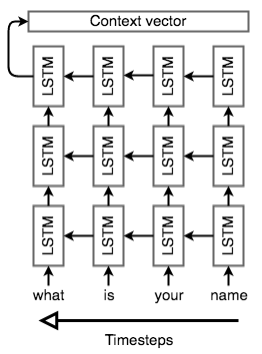
\includegraphics[width=\textwidth]{images/encoder.png}
         \caption{Encoder}
         \label{fig:encoder}
     \end{subfigure}
    %  \hfill
     \begin{subfigure}[b]{0.25\textwidth}
         \centering
         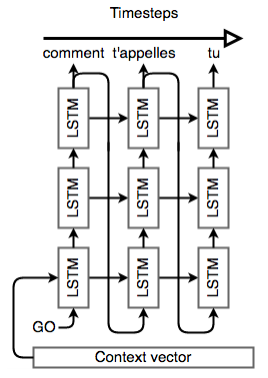
\includegraphics[width=\textwidth]{images/decoder.png}
         \caption{Decoder}
         \label{fig:decoder}
     \end{subfigure}
        \caption{Encoder-Decoder architecture using LSTM for seq2seq model}
        \label{fig:enc_dec}
\end{figure}

\paragraph{Attention} A problem with general encoder-decoder model is that they give equal importance to all the parts of input sequence. Also, the input sequence is compressed into a single context vector which creates the bottleneck problem, where a long information is tried to be kept into one small representation. 

A solution to this problem was proposed in the work \cite{bahdanau2014neural} introducing a new mechanism called Attention. Attention aligns the output at each decoding step to the whole input sequence in order to learn the most important part of the input aligning with the current step output by providing an attentive output.

Let's say we have calculated the encoding hidden states $(h_{1},  h_{2}, \cdots, h_{n})$ for the input sequence $(x_{1}, x_{2}, \cdots, x_{n})$ during the calculation of context vector $Z$. For a decoder hidden state $s_{t}$ on timestep $t$, we get attention score $e^{t}$ as follows:

\begin{equation}
    \label{eq:att_score}
        e^{t} = [s^{T}_{t}h_{1}, \cdots, s^{T}_{t}h_{n}]
\end{equation}

We take the softmax of these scores to get the attention distribution at timestep $t$.

\begin{equation}
    \label{eq:att_dist}
        \alpha^{t} = softmax(e^{t})
\end{equation}

The attention output $a_{t}$ is then calculated as the weighted sum of encoder hidden state using $\alpha^{t}$:

\begin{equation}
    \label{eq:att_out}
        a_{t} = \sum_{i=1}^{n} \alpha_{i}^{t}h_{i}
\end{equation}

Finally, we concatenate the attention output $a_{t}$ with decoder hidden state $s_{t}$ and proceed to calculate the negative log loss same as the non-attention decoder model.

\subsubsection{Contextual Word Embeddings}\label{sec:context_we}
As discussed in \cref{sec:word_emb}, the word embeddings generated by algorithms like word2vec \cite{mikolov2013distributed} and GloVe \cite{pennington2014glove} lacks the contextual awareness and fail to differentiate a word with different sense. For example, word $get$ has thirty different senses (meaning) in wordnet \footnote{\url{https://wordnet.princeton.edu/}} based on the different contexts. But if we use pre-trained word embeddings to generate the vector representation of $get$, it will be same for all the thirty times and we will loose the semantic information. 

A new trend of transfer learning came in Deep Learning based NLP with the introduction works like ELMo \cite{peters2018deep} and ULMFiT \cite{howard2018universal} where language models are used to learn the nuances of the language grammar and then the pre-trained language model is then fine-tuned on a task specific dataset to achieve better results.

\begin{figure}
    \centering
    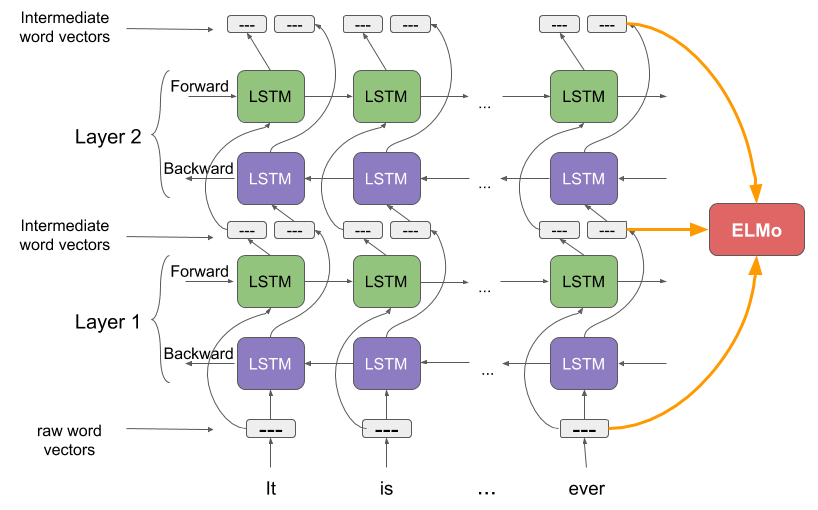
\includegraphics[width=0.75\textwidth]{images/elmo.png}
    \caption{ELMo Vector Representation}
    \label{fig:elmo}
\end{figure}

\paragraph{ELMo} stands for Embeddings Learned from Language Models \cite{peters2018deep} uses a bidirectional language model to capture the context of a word in a sentence from both sides (left to right and vice-versa). ELMo uses an character-level CNN to convert raw text into a word vector which is then fed into a bidirectional language model. The ouput of this BiLM is then sent to the next layer of BiLM to form a set of intermediate word vectors. The final output of ELMo is the weighted sum of raw vectors and the intermediate vectors formed from two layers of the BiLMs. The two language models used here are based on LSTM architectures. An illustration of ELMo is shown is \cref{fig:elmo} \footnote{Taken from \url{https://www.analyticsvidhya.com/blog/2019/03/learn-to-use-elmo-to-extract-features-from-text/}}.

ELMo achieved 9\% error reduction on the SQuAD (question-answering) dataset compared to then state-of-the-art, 16\% on Ontonotes SRL dataset, 10\% on Ontonotes coreference dataset and 4\% on CoNLL 2003 dataset. It paved a huge path in the success of contextualized word representations for different tasks in NLP.

\paragraph{ULMFiT} stands for Universal Language Model Fine Tuning, introduced the way of applying transfer learning on text classification problem \cite{howard2018universal}. It does so in three main steps: first, train an general domain language model on large corpus of text (mainly Wikipedia); second, fine tune the language model on task specific target dataset; and third, use the again fine tune the fine-tuned language model as classifier by adding a softmax activation on top with target dataset. An illustration of the three steps of ULMFiT is shown in \cref{fig:ulmfit_steps}.

% \begin{figure}
%     \centering
%     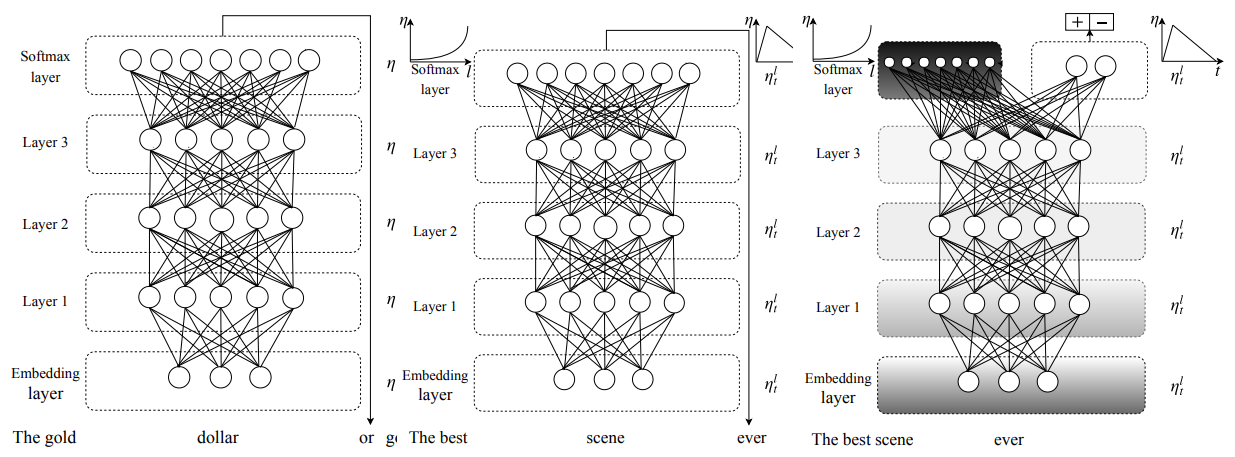
\includegraphics[width=\textwidth]{images/ulmfit.png}
%     \caption{ULMFiT Steps}
%     \label{fig:ulmfit}
% \end{figure}

\begin{figure}
     \centering
     \begin{subfigure}[b]{0.3\textwidth}
         \centering
         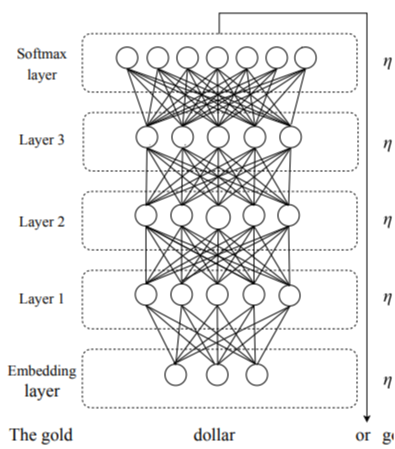
\includegraphics[width=\textwidth]{images/ulm1.png}
         \caption{LM Training}
         \label{fig:lm_train}
     \end{subfigure}
    %  \hfill
     \begin{subfigure}[b]{0.3\textwidth}
         \centering
         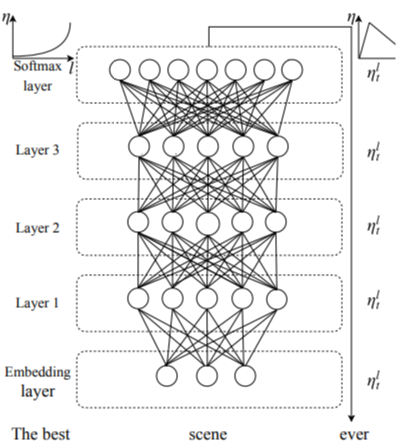
\includegraphics[width=\textwidth]{images/ulm2.png}
         \caption{LM Fine-Tuning}
         \label{fig:lm_ft}
     \end{subfigure}
    %  \hfill
     \begin{subfigure}[b]{0.3\textwidth}
         \centering
         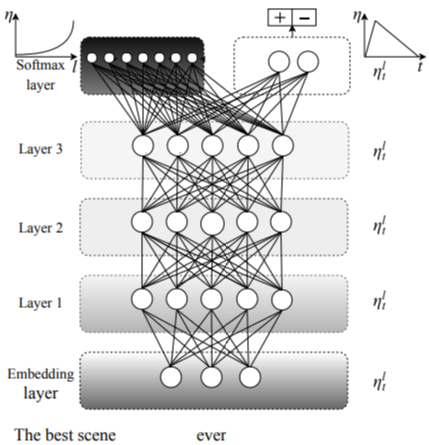
\includegraphics[width=\textwidth]{images/ulm3.png}
         \caption{Classifier Training}
         \label{fig:lm_classif}
     \end{subfigure}
        \caption{ULMFiT Steps \cite{howard2018universal}}
        \label{fig:ulmfit_steps}
\end{figure}


ULMFiT achieved better results for text classification on six different datasets ranging from topic classification to sentiment analysis. It did so by learning the general rules of grammar from huge corpus of text and then transferring that learning with fine tuning on a task-specific dataset providing better results than state-of-the-arts \cite{howard2018universal}.

\subsubsection{Transformers}\label{sec:transformers}
Almost all of the models we discussed have recurrent behaviour, which can not be trained parallely. This imposes a huge problem of time taken to train a model from scratch. In the work \cite{vaswani2017attention}, authors proposed a new neural architecture called Transformers which uses a combination of self attention and feed-forward network in its encoder-decoder model and doesn't require any recurrent or convolutional elements. This new seq2seq model was a huge success where it gained better performance on various sequential NLP tasks. To name one, it improved the machine translation performance by 10\% on WMT EN-FR and WMT EN-DE datasets. It also reduced the training time by large margin benefiting its non-recurrent nature \cite{vaswani2017attention}.

The success of transformer architecture paved the way for development of new models to solve the sequential tasks. It helped NLP researchers to utilize its non-recurrent nature in transfer learning where the transformer is used for general pre-training of a language model on large corpus of text which can be used for fine-tuning on domain specific dataset for downstream tasks. An encoder-decoder model of Transformer architecture is shown in the \cref{fig:trans}.

\begin{figure}
    \centering
    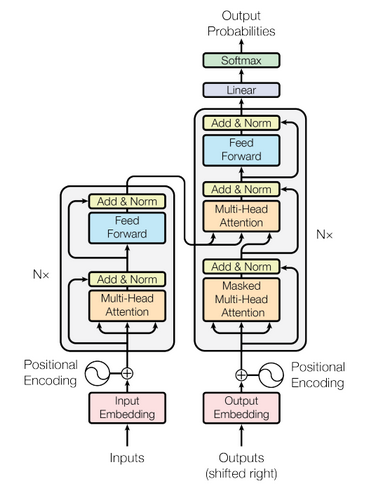
\includegraphics[width=0.5\textwidth]{images/transformer.png}
    \caption{Transformer architecture \cite{vaswani2017attention}.}
    \label{fig:trans}
\end{figure}

\paragraph{Generative Pre-Training}
One of the earliest works in using Transformers for pre-training of language model was presented in \cite{radford2018improving}. Following the idea from ELMo \cite{peters2018deep}, authors proposed a language model using transformer decoder trained on large corpus and then fine-tuned on task specific dataset. The main difference of GPT from ELMo is that ELMo uses two independent LSTM language models to caputre the forwards and backward context whereas in case of GPT, it uses a uni-directional multi-layer transformer language model capable of capturing context due to its attentive nature.

ELMo takes a feature based approach of feeding feature vectors for different tasks into different models, whereas GPT takes a fine-tuning based approach where same language model trained on huge corpus is fine-tuned for downstream tasks without changing the architecture. An illustration of a GPT model used for pre-training is shown in \cref{fig:gpt} \footnote{Taken from \url{https://openai.com/blog/language-unsupervised/}}.

\begin{figure}
    \centering
    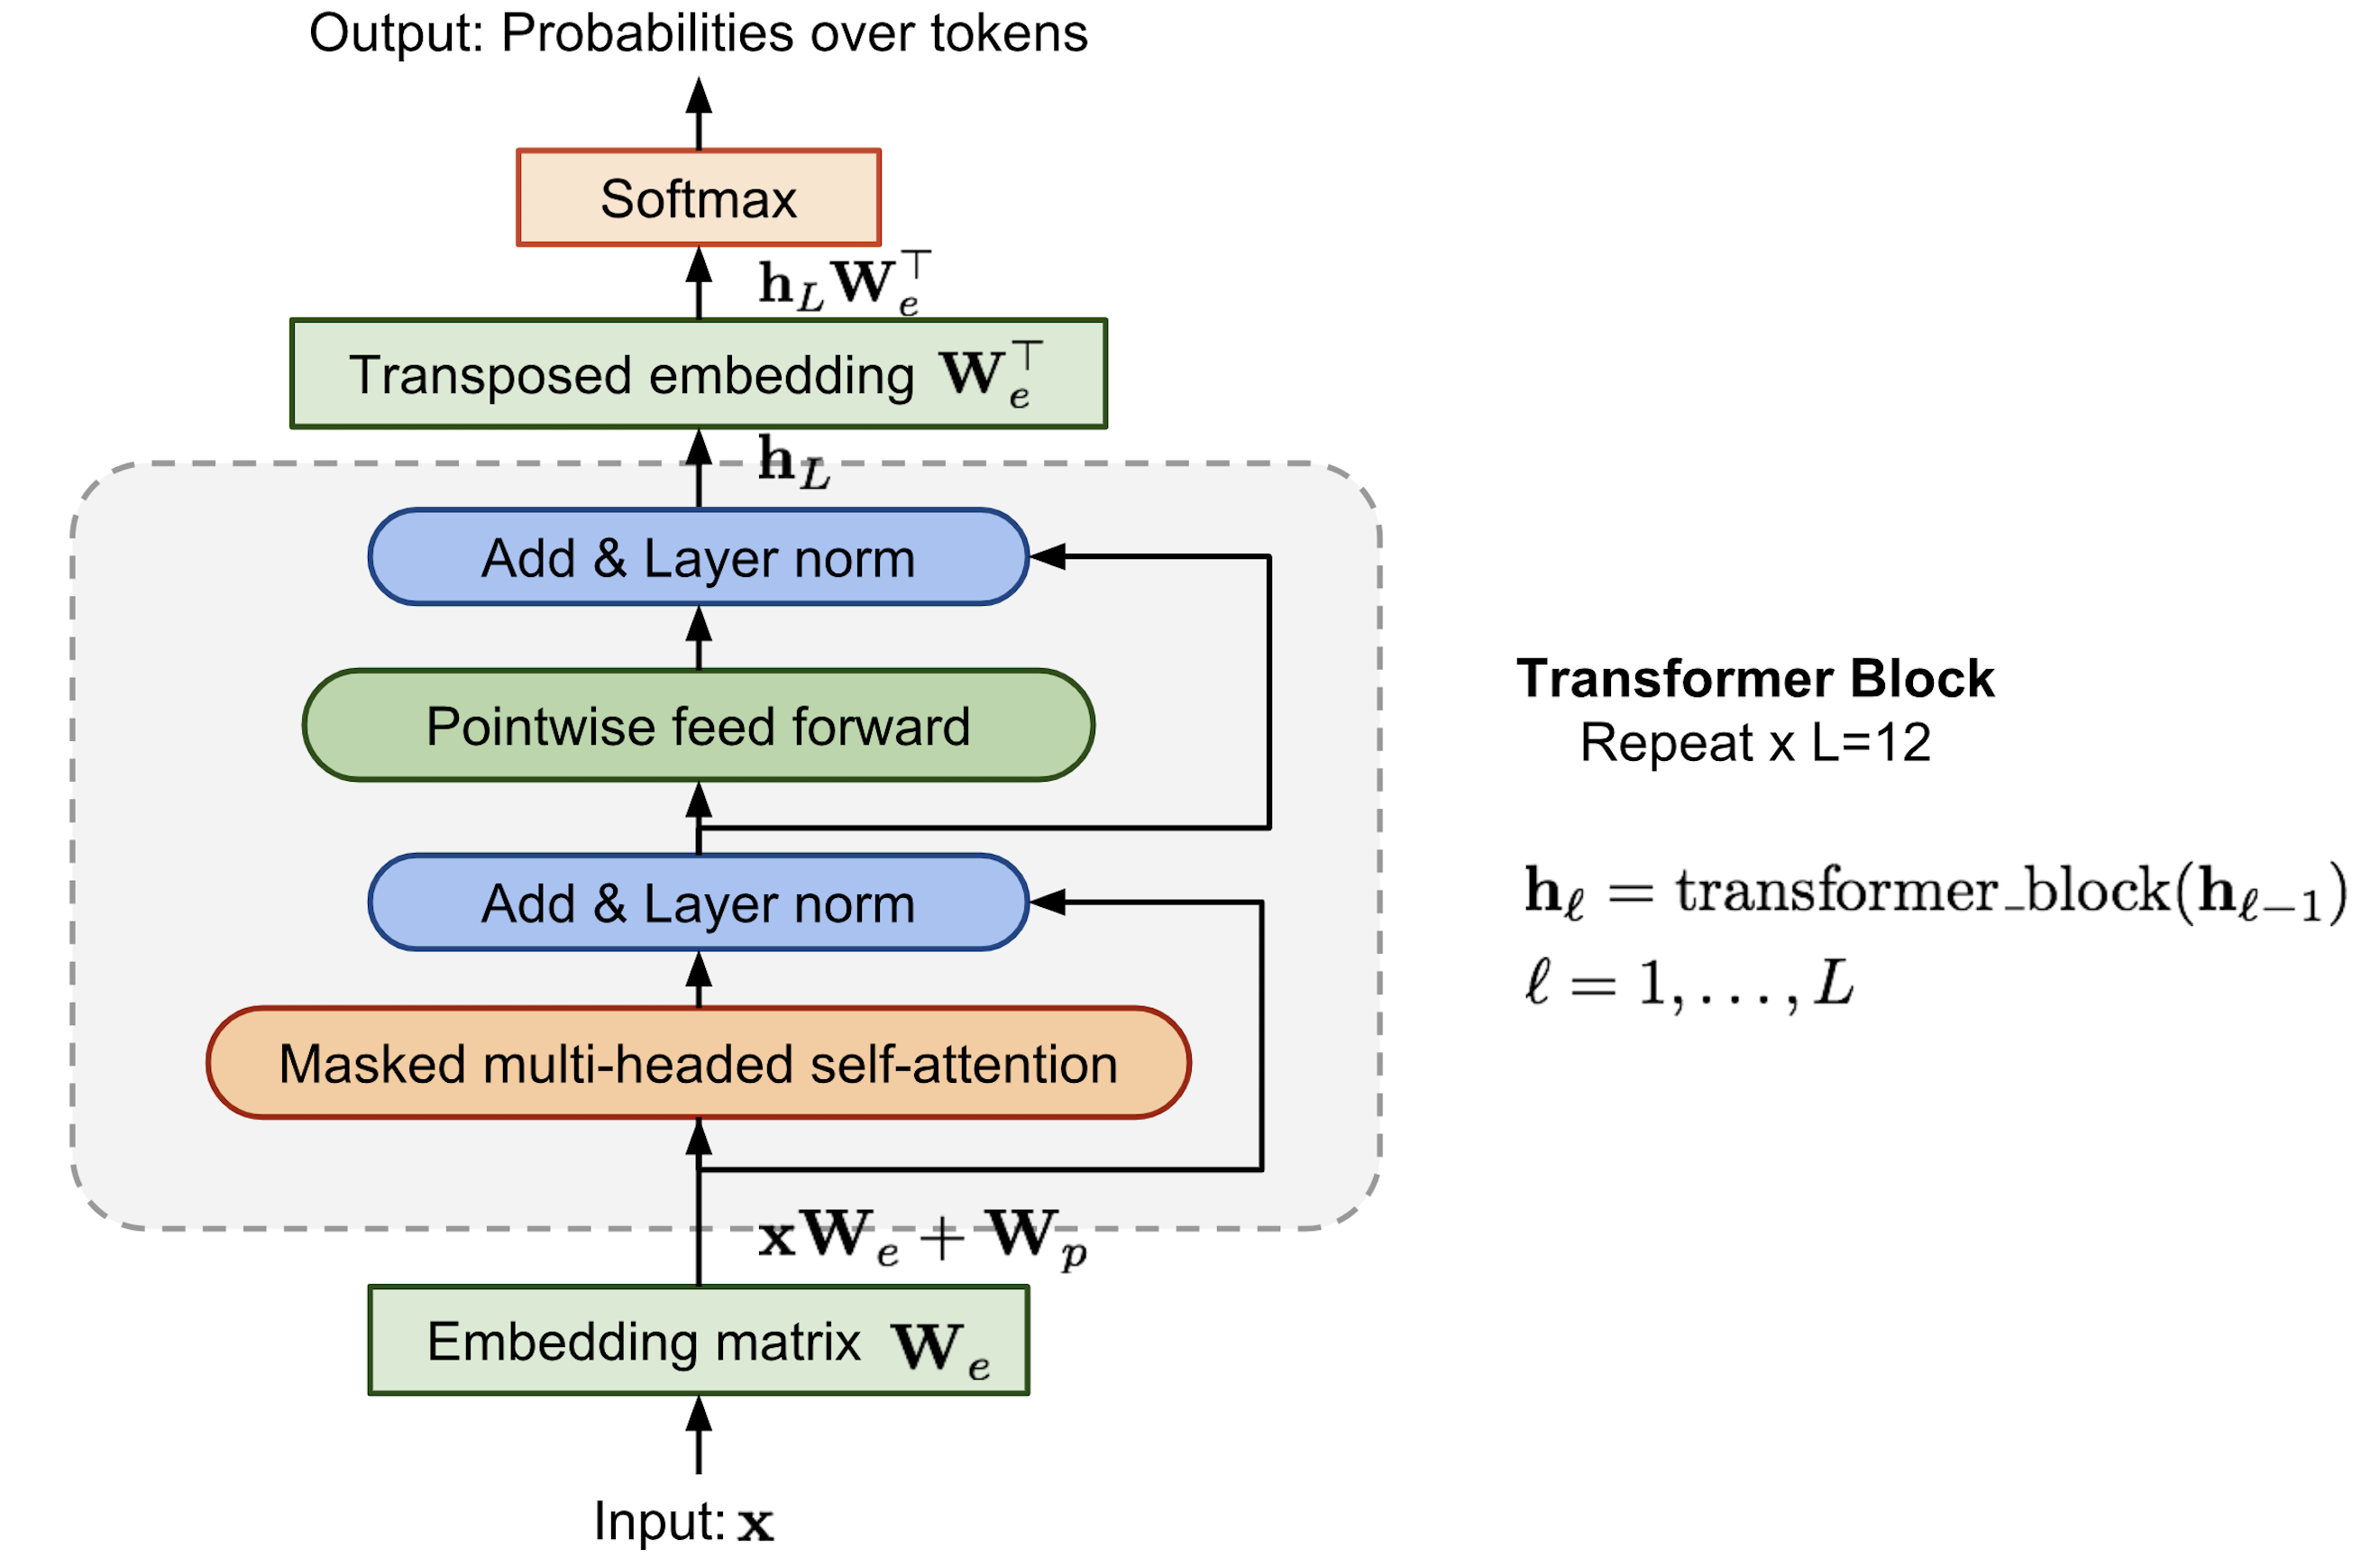
\includegraphics[width=0.75\textwidth]{images/GPT.png}
    \caption{GPT architecture.}
    \label{fig:gpt}
\end{figure}

\paragraph{Bidirectional Encoder Representation from Transformers}
BERT \cite{devlin2018bert} is another example of the success of transfer learning in NLP. BERT is a bidirectional transformer language model trained on a large text corpus that can be fine-tuned on any domain specific dataset for the downstream tasks like text classification or named entity recognition. BERT mainly differs from other models like GPT and ELMo because of the pre-training tasks used during the unsupervised training of language model. It involves two tasks; first, Masked Language Model (MLM) \cite{taylor1953cloze} or prediction of the masked word in a sentence, and second, prediction of next sentence from the corpora.

For the first task of Masked Language Model, let’s say we have a sentence ‘Boris Johnson is the Prime Minister of UK’. So instead of training for prediction of next word in the sentence as a general Language Model, BERT pre-training replaces 15\% of the words with a [MASK] token and learns to predict the correct word at the position of [MASK] token. In the second task of Next Sentence Prediction, the model is trained to learn the relationship between sentences where for a given sentence pair A \& B, the model is asked to predict if the sentence B is actually the next sentence that comes after A or not?

BERT improved the fine-tuning based approach of GPT by using a bidirectional transformer for masked language modelling by learning the both left and right context which is a huge improved over GPT's unidirectional approach specially for token-level tasks like Question Answering where the answer depends on both left and right contexts. An illustrated diagram of BERT pre-training and fine-tuning is shown in \cref{fig:bert1}. 
% A visual comparison between BERT, GPT and ELMo architectures presented in the work \cite{devlin2018bert} is shown in \cref{fig:bert2}.

\begin{figure}
    \centering
    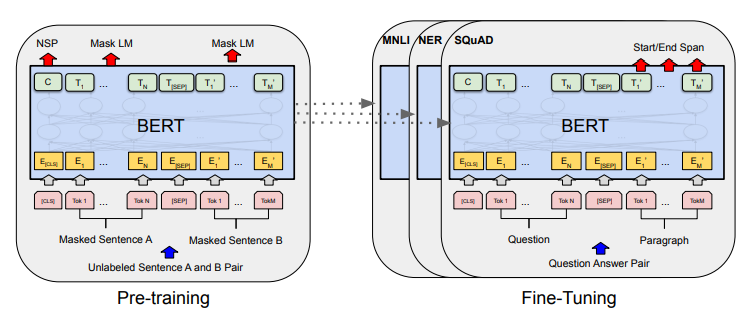
\includegraphics[width=0.75\textwidth]{images/bert1.png}
    \caption{BERT \cite{devlin2018bert}}
    \label{fig:bert1}
\end{figure}


% \begin{figure}
%     \centering
%     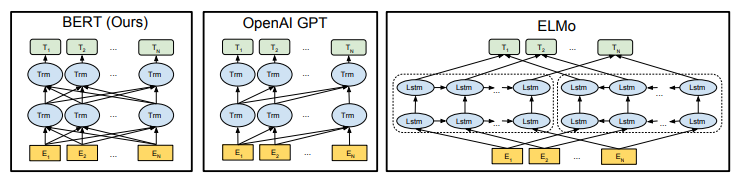
\includegraphics[width=\textwidth]{images/bert2.png}
%     \caption{BERT, GPT and ELMo \cite{devlin2018bert}}
%     \label{fig:bert2}
% \end{figure}
